\chapter{Analiza wymagań}

\section{Wstęp}

%TODO Alternatywna wersja 

Wraz z rozwojem handlu konieczne stało się stworzenie miejsca w którym towary
będą składowane przed zakupem przez klienta. W przypadku małych magazynów to
pracownicy są w stanie nim efektywnie zarządzać i efektywnie wyszukiwać 
znajdujące się w nim towary. Jednak co dzieje się w przypadku, gdy liczba towarów
przechowywanych w magazynie jest bardzo duża? Konieczne staje się stworzenie
systemu który umożliwi pracownikom prostsze i bardziej efektywne zarządzanie
towarami znajdującymi się w magazynie.

Głównym zadaniem systemu do zarządzania magazynem jest przechowywanie ilości
poszczególnych towarów, odznaczanie dostaw jak i również sprzedaży
towarów klientom. Powinien również przechowywać niezbędne informacje o
dostawcach, towarach oraz klientach.

\subsection{Przeznaczenie systemu}

Głównym zadaniem systemu jest ułatwienie zarządzania magazynem pracownikom
magazynu, poprzez umożliwienie zarządzania klientami, dostawcami, towarami a
także zamówieniami sprzedaży jak i zakupu. System ten nie jest specjalizowany
pod konkretną dziedzinę handlu -- ma on umożliwiać przechowywanie i
zarządzanie informacjami o towarach dowolnego typu. 

\subsection{Architektura systemu}

W obecnie tworzonych systemach spotyka się dwie podstawowe struktury:
architekturę klient-serwer oraz architekturę trójwarstwową.
W architekturze klient-serwer, która była szczególnie popularna w
latach dziewięćdziesiątych ubiegłego wieku, wyróżnia się
dwie warstwy: 
\begin{itemize}
 \item aplikację użytkownika (\emph{klient});
 \item system zarządzania bazą danych (\emph{serwer}).
\end{itemize}

Struktura ta sprawdza się dla prostych systemów, których zadaniem jest
zapisywanie, odczytywanie oraz aktualizacja danych. Problem
pojawia się jednak w przypadku, gdy dane muszą być przetwarzane w
nietrywialny sposób, przy uwzględnieniu dziedziny problemu (ang. \emph{domain
logic}) modelowanego zagadnienia. Realizacja obliczeń w warstwie klienta,
której głównym zadaniem jest prezentacja informacji użytkownikowi, może
znacząco wpływać na jego komfort pracy oraz powodować problemy związane z
duplikacją kodu źródłowego aplikacji.
Natomiast umieszczenie logiki aplikacji po stronie serwera bardzo często narzuca
przygotowanie programu w środowisku specyficznym dla danego systemu zarządzania
bazami danych. 

Problemy te zmusiły projektantów aplikacji do wydzielenia jeszcze jednego
poziomu, który jest odpowiedzialny za logikę operacji na danych. W
architekturze trójwarstwowej uwzględnione są następujące warstwy:
\begin{itemize}
 \item warstwa prezentacji;
 \item warstwa aplikacji;
 \item warstwa źródła danych.
\end{itemize}

\begin{figure}[h]
    \begin{center}
    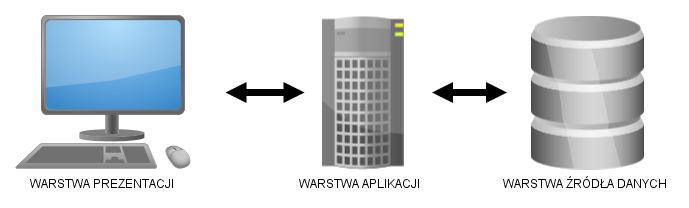
\includegraphics[scale=0.5]{../img/arch-3warstw.png}
    \end{center}
    \label{fig:arch3warstw}
    \caption{Schemat architektury trójwarstwowej}
\end{figure}
\FloatBarrier
W przypadku realizowanego systemu do obsługi magazynu zastosowana będzie
architektura trójwarstwowa.

\section{Aktorzy}

Aktorzy w zaprojektowanym systemie zostali podzieleni na dwie grupy: aktorów
osobowych oraz aktorów nieosobowych. Do aktorów osobowym można zaliczyć
wszystkich użytkowników projektowanego systemu, aktorami nieosobowymi są
natomiast wszystkie systemy zewnętrzne współpracujące z projektowanym systemem.
Poniższy diagram przedstawia hierarchię aktorów osobowych w systemie:

\begin{figure}[h]
    \begin{center}
    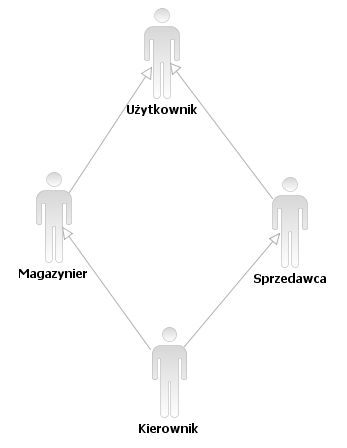
\includegraphics[scale=0.75]{../img/diagramDziedziczenia.png}
    \end{center}
    \label{fig:diagramDziedziczenia}
    \caption{Diagram przedstawiający aktorów w systemie}
\end{figure}
\FloatBarrier

\section{Wymagania funkcjonalne}

Niniejsze rozdział zawiera wymagania funkcjonalne jakie powinien spełniać
projektowany system. Wymagania te zostały podzielone na odpowiednie grupy wymagań.
Grupy wymagań zawierają bardziej szczegółowe wymagania, takie jak edycja czy
usuwanie danych. W tabeli umieszczone zostały również informacje o priorytecie
wymagania oraz ryzyku realizacji i aktorach.

%\arrayrulecolor{line}
%\rowcolors{2}{cell}{white}

\begin{table}[ht]
	 \begin{center}
% 	    \rowcolors{1}{}{light-blue}
	    \begin{tabular}{| l | l | l | l | l |}%\toprule
	    	\hline
		    \textbf{LP.} & \textbf{Nazwa}  & \textbf{Priorytet} & \textbf{Ryzyko} &
		    \textbf{Nazwa aktora} \\
		    \hline
			1 & Zarządzanie pracownikami & wysoki & niskie & kierownik \\
		    1.1 & Dodawanie pracownika & wysoki & niskie & kierownik \\
		    1.2 & Edycja danych pracownika & wysoki & niskie & kierownik \\ 	
		    1.3 & Usuwanie danych pracownika & wysoki &niskie & kierownik \\
		    \hline
		    2 & Zarządzanie danymi towarów & wysoki & niskie & magazynier \\
		    2.1 & Dodawanie towaru & wysoki &  niskie & magazynier \\
		    2.2 & Edycja opisu towaru & wysoki & niskie & magazynier \\
		    2.3 & Usuwanie danych towaru & wysoki & niskie & magazynier \\
            2.4 & Korekta stanu towaru & wysoki & niskie & magazynier \\
		    \hline
		   	3 & Zarządzanie danymi kontrahentów & wysoki & niskie & użytkownik \\
		   	3.1 & Dodawanie kontrahenta & wysoki & niski & użytkownik \\
		   	3.2 & Edycja danych kontrahenta & wysoki & niskie & użytkownik \\
		   	3.3 & Usuwanie danych kontrahenta & średni & niskie & użytkownik \\
		   	\hline
            4 & Przyjęcie na magazyn & wysoki & niskie & magazynier \\
		   	4.1 & Tworzenie dokumentu przejęcia towaru & wysoki & niskie & magazynier \\
		   	4.2 & Edycja dokumentu przyjęcia towaru & wysoki & niskie & magazynier \\
		   	4.3 & Usuwanie dokumentu przyjęcia towaru & wysoki & niskie & magazynier \\
		   	4.4 & Realizacja przyjęcia towaru & wysoki & niskie & magazynier \\
		   	4.5 & Korekta przyjęcia towaru & średni & niskie & magazynier \\
            4.5.1 & Tworzenie dokumentu korekty przyjęcia towaru & średni & niskie & magazynier \\
            4.5.2 & Edycja dokumentu przyjęcia towaru & średni & niskie & magazynier \\
            4.5.3 & Usuwanie dokumentu przyjęcia towaru & średni & niskie & magazynier \\
            4.5.4 & Realizacja korekty przyjęcia towaru & średni & niskie & magazynier \\ 
            \hline
		   	5 & Wydanie z magazynu & wysoki & niskie & sprzedawca \\
		   	5.1 & Tworzenie dokumentu wydania towaru & wysoki & niskie & sprzedawca \\
		   	5.2 & Edycja dokumentu wydania towaru & średni & niskie & sprzedawca \\
		   	5.3 & Usuwanie dokumentu wydania towaru & wysoki & niskie & sprzedawca \\
		   	5.4 & Realizacja wydania towaru & wysoki & niskie & sprzedawca \\
		   	5.5 & Korekta wydania towaru & średni & niskie & sprzedawca \\
            5.5.1 & Tworzenie dokumentu korekty wydania towaru & średni & niskie & sprzedawca \\
            5.5.2 & Edycja dokumentu wydania towaru & średni & niskie & sprzedawca \\
            5.5.3 & Usuwanie dokumentu wydania towaru & średni & niskie & sprzedawca \\
            5.5.4 & Realizacja korekty wydania towaru & średni & niskie & sprzedawca \\ 
		   	\hline
		   	6 & Zarządzanie raportami & średni & niskie & kierownik \\
		   	6.1 & Generowanie raportów o wydanych towarach & średni & niskie & kierownik \\
		   	6.2 & Generowanie raportów o przyjętych towarach & średni & niskie & kierownik \\
		   	\hline
	    \end{tabular}
	\end{center}
\end{table}
\FloatBarrier

\section{Wymagania niefunkcjonalne}

Rozdział ten zawiera wymagania niefunkcjonalne dotyczące projektowanego systemu.
Wymagania zostały podzielone na kilka grup, przy każdym z wymagań został
określony priorytet oraz ryzyko.

\begin{table}[h]
	\begin{center}
		\begin{tabular}{| l | l | l | l |}
			\hline
			\textbf{Lp.} & \textbf{Nazwa} & \textbf{Priorytet} & \textbf{Ryzyko} \\
			\hline
			1 & Bezpieczeństwo & wysoki & niskie \\
			1.1 & Mechanizm uwierzytelniania użytkowników za pomocą & wysoki & niskie \\
			& loginu i hasła & & \\
			1.2 & Zróżnicowanie uprawnień do korzystania z systemu & wysoki & niskie \\
			1.3 & Zapisywanie historii przeprowadzanych transakcji & wysoki & niskie \\
			1.4 & Szyfrowanie haseł w bazie danych funkcją skrótu & wysoki & niskie \\
			\hline
			2 & Dostępność & wysoki & niskie \\
			2.1 & Dostępność systemu co najmniej 98\% w skali dnia & wysoki & niskie \\ 
			2.2 & Dostępność przez przeglądarkę & wysoki & niskie \\
			\hline
			3 & Elastyczność & wysoki & niskie \\
			3.1 & Architektura systemu umożliwia łatwą rozbudowę  & wysoki & niskie \\
			& i konserwacje & & \\
			3.2 & Możliwość integracji z innymi systemami używanymi & wysoki & niskie \\
			& w firmie & & \\
			
			\hline
			4 & Niezawodność & wysoki & niskie \\
			4.1 & Maksymalny czas powstania po awarii 2h & wysoki & niskie \\
			4.2 & Odtwarzanie uszkodzonych danych na podstawie & wysoki	& niskie \\
			& kopii zapasowych & & \\
			4.3 & Wykonywanie kopii zapasowych danych & wysoki & niskie \\
			\hline
			5 & Użyteczność & wysoki & niskie \\
			5.1 & Intuicyjny sposób obsługi systemy & wysoki & niskie \\
			5.2 & Przejrzysty system pomocy & wysoki & niskie \\
			\hline
			6 & Wydajność & wysoki & niskie \\
			6.1 & Przechowywanie informacji o transakcjach przez 3 lata & wysoki & niskie
			\\
			6.2 & Umożliwienie równoczesnej pracy przez 200 użytkowników & wysoki &
			niskie
			\\
			\hline
		\end{tabular}
	\end{center}
\end{table}
\FloatBarrier

\section{Specyfikacja przypadków użycia na poziomie ogólnym}

Dwa podstawowe zadania kierownika to zarządzanie pracownikami (innymi użytkownikami systemu) oraz zarządzanie raportami. Posiada on największe uprawnienia
w systemie. Może dodawać i usuwać pracowników, a także nadawać im uprawnienia. Kierownik zajmuje się generowaniem raportów wydanych oraz przyjętych towarów.  Diagram przedstawiający przypadki użycia kierownika znajduje
się na rysunku \ref{fig:kierownikUseCase}.

Magazynier jest osobą odpowiedzialną za odwzorowanie aktualnego stanu
magazynu w systemie. Wprowadza dane towarów do systemu, a także
aktualizuje ich stan. Ponadto zarządza on przyjęciami towaru do
magazynu oraz danymi kontrahentów.  Zadaniem magazyniera jest
prowadzenie ewidencji kontrahentów, dodawanie nowych oraz usuwanie
tych, z którymi zakończono współpracę. Magazynier kontroluje
przyjmowanie towarów do magazynu.  W razie potrzeby może zwrócić
przyjęty towar. Diagram przedstawiający opisane przypadki użycia
został zaprezentowany na rysunku \ref{fig:magazynierUseCase}.

Sprzedawca pośredniczy w kontaktach z kontrahentem i zarządza procesem
sprzedaży towarów. Przyjmuje on zamówienia (wykonuje operacje wydania
towaru z magazynu) i dodaje je do bazy, aktualizując jednocześnie dane
klientów. Sprawuje kontrolę nad realizacją wydania towaru z magazynu,
a w razie potrzeby może przyjąć zwrócony towar. Do zadań sprzedawcy
należy prowadzenie ewidencji kontrahentów, aktualizowanie informacji o
nich oraz usuwanie starych. Przypadki użycia sprzedawcy zostały
zaprezentowane na diagramie \ref{fig:sprzedawcaUseCase}.

\begin{figure}[ht]
  \begin{center}
    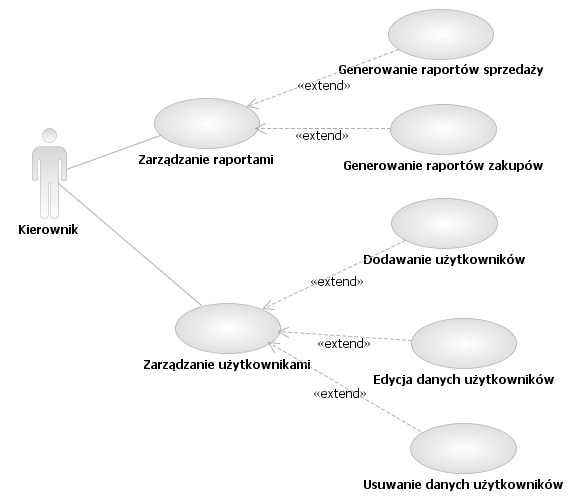
\includegraphics[angle=-90,scale=0.8]{../img/kierownikUseCase.png}
  \end{center}
  \caption{Diagram przypadków użycia kierownika}
  \label{fig:kierownikUseCase}
\end{figure}

\begin{figure}[ht]
  \begin{center}
    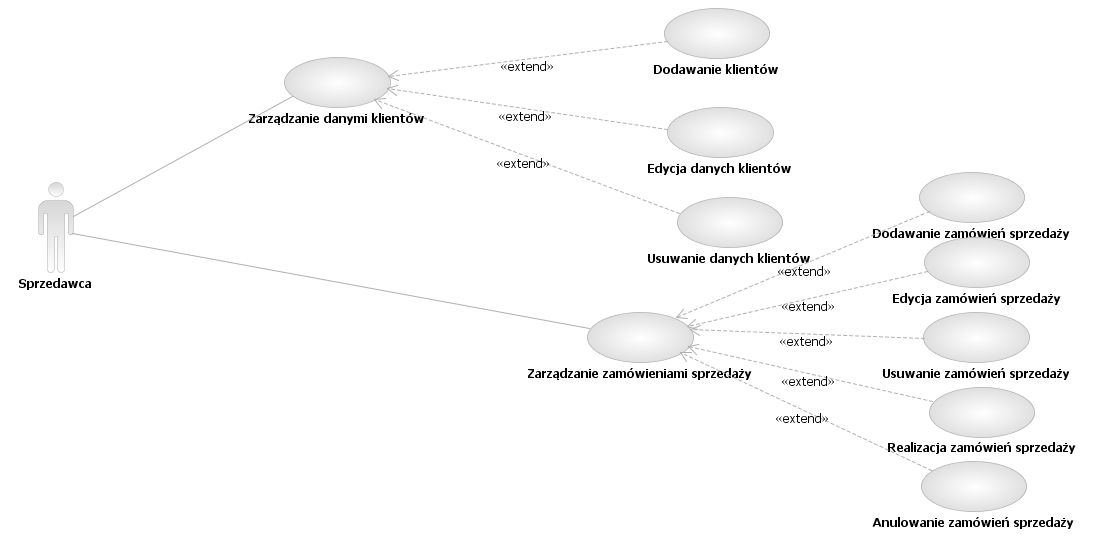
\includegraphics[angle=-90,scale=0.75]{../img/sprzedawcaUseCase.png}
  \end{center}
  \caption{Diagram przypadków użycia sprzedawcy}
  \label{fig:sprzedawcaUseCase}
\end{figure}


\begin{figure}[ht]
  \begin{center}
    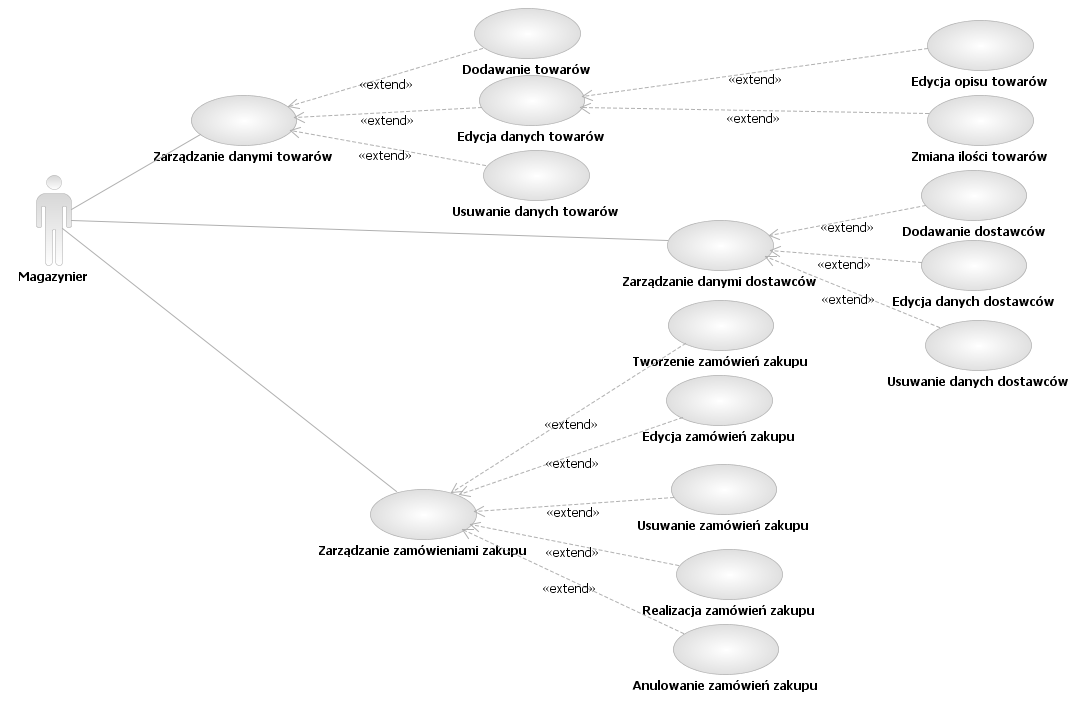
\includegraphics[angle=-90,scale=0.7]{../img/magazynierUseCase.png}
    \caption{Diagram przypadków użycia magazyniera}
    \label{fig:magazynierUseCase}
  \end{center}
\end{figure}

